\chapter{Assignment-Complex Numbers}
\section{MCQ}
\begin{enumerate}
	\item $\left. \right. $
	\begin{answer}
		\begin{align*}
	\frac{1+i \sqrt{3}}{\sqrt{3}+i}&=\frac{(1+i \sqrt{3})(\sqrt{3}-i)}{(\sqrt{3}+i)(\sqrt{3}-i)}=\frac{2 \sqrt{3}+2 i}{4}=\frac{\sqrt{3}}{2}+\frac{1}{2} i\\
\intertext{	Since both the real and complex parts are greater than zero, hence the argument is the acute angle given by $\tan ^{-1}\left|\frac{\frac{1}{2}}{\frac{\sqrt{3}}{2}}\right|=\tan ^{-1} \frac{1}{\sqrt{3}}=\frac{\pi}{6}$}
		\end{align*}
		So the correct answer is \textbf{Option (c)}
	\end{answer}
\item $\left. \right. $	
	\begin{answer}
		\begin{align*}
		a+i b&=\frac{1-i x}{1+i x} \Rightarrow a-i b=\frac{1+i x}{1-i x}\\
		\therefore \quad(a+i b)(a-i b)&=\frac{1-i x}{1+i x} \cdot \frac{1+i x}{1-i x} \Rightarrow a^{2}+b^{2}=\frac{1+x^{2}}{1+x^{2}}=1
		\end{align*}
		So the correct answer is \textbf{Option (a)}
	\end{answer}
\item $\left. \right. $	
	\begin{answer}
		\begin{align*}
		|z|=\sqrt{(1-\cos \theta)^{2}+\sin ^{2} \theta}=\sqrt{2-2 \cos \theta}=\sqrt{4 \sin ^{2} \frac{\theta}{2}}=2\left|\sin \frac{\theta}{2}\right|
		\end{align*}
		So the correct answer is \textbf{Option (c)}
	\end{answer}
\item $\left. \right. $		
	\begin{answer}
		\begin{align*}
		|z|=\frac{1}{|2+3 i|^{2}}=\frac{1}{\left(\sqrt{2^{2}+3^{2}}\right)^{2}} \quad|z|=\frac{1}{13}
		\end{align*}
		So the correct answer is \textbf{Option (a)}
	\end{answer}
\item $\left. \right. $		
	\begin{answer}
		\begin{align*}
		x_{1} \cdot x_{2} \cdot x_{3} \ldots .&\text{ to infinity }=\left(\cos \frac{\pi}{2}+i \sin \frac{\pi}{2}\right)\left(\cos \frac{\pi}{2^{2}}+i \sin \frac{\pi}{2^{2}}\right)\left(\cos \frac{\pi}{2^{3}}+i \sin \frac{\pi}{2^{3}}\right) \ldots \infty\\
		&=\cos \left(\frac{\pi}{2}+\frac{\pi}{2^{2}}+\frac{\pi}{2^{3}}+\ldots\right)+i \sin \left(\frac{\pi}{2}+\frac{\pi}{2^{2}}+\frac{\pi}{2^{3}}+\ldots\right)=\cos \left(\frac{\frac{\pi}{2}}{1-\frac{1}{2}}\right)+i \sin \left(\frac{\frac{\pi}{2}}{1-\frac{1}{2}}\right)\\
		&=\cos \pi+2 i \sin \pi=-1
		\end{align*}
		So the correct answer is \textbf{Option (c)}
	\end{answer}
\item $\left. \right. $		
	\begin{answer}
		\begin{align*}
		|z|&=\left|z-\frac{4}{z}+\frac{4}{z}\right| \leq\left|z-\frac{4}{z}\right|+\left|\frac{4}{z}\right|
		\intertext{Using triangle in equinity}
		\Rightarrow \quad&|z| \leq 2+\frac{4}{|z|} \quad\text{ since } \left|z-\frac{4}{z}\right|=2\\
		&\Rightarrow \quad|z|^{2}-2|z|-4 \leq 0 \Rightarrow(|z|-1+\sqrt{5})(|z|-1-\sqrt{5}) \leq 0 \Rightarrow(1-\sqrt{5}) \leq|z| \leq 1+\sqrt{5}\\
		\text{Thus }&\text{the maximum value of }\text{$|z|$ is $1+\sqrt{5}$}
		\end{align*}
		So the correct answer is \textbf{Option (b)}
	\end{answer}
\item $\left. \right. $		
\begin{answer}
	\begin{align*}
	&1+\sum_{k=0}^{14}\left\{\cos \frac{(2 k+1) \pi}{15}+i \sin \frac{(2 k+1) \pi}{15}\right\}\\
	&=1+\sum_{k=0}^{14} e^{i \frac{(2 k+1) \pi}{15}}=1+\sum_{k=0}^{14} \alpha^{2 k+1}\qquad
\text{	where }\alpha=e^{i \frac{\pi}{15}}\\
&=1+\left(\alpha+\alpha^{3}+\alpha^{5}+\ldots \alpha^{29}\right)=1+\alpha\left(\frac{1-\left(\alpha^{2}\right)^{15}}{1-\alpha^{2}}\right)\\
&=1+\alpha\left(\frac{1-\alpha^{30}}{1-\alpha^{2}}\right)=1+\alpha\left(\frac{1-1}{1-\alpha^{2}}\right)=1 \quad\left[\right.\text{ since }\left.\quad \alpha^{30}=e^{\mathrm{i} 2 \pi}=1\right]
	\end{align*}
	So the correct answer is \textbf{Option (c)}	
\end{answer}	
\item $\left. \right. $
\begin{answer}
	\begin{align*}
	\text{Let }z&=x+i y,\text{ then}\\
	|z+4|^{2}-|z-4|^{2}&=8 \Rightarrow 4 \operatorname{Re}(4 z)=8
\intertext{	where $\operatorname{Re}(4 z)$ is the real part of the complex number $4 z$}
\Rightarrow \quad \operatorname{Re}(z)&=\frac{1}{2} \Rightarrow x=\frac{1}{2},\text{ which is a straight line parallel to the $y$-axis.}
	\end{align*}
	So the correct answer is \textbf{Option (b)}
\end{answer}	
\item $\left. \right. $	
	\begin{answer}
		\begin{align*}
		\intertext{we have}
		\left|\begin{array}{ccc}6 i & -3 i & 1 \\ 4 & 3 i & -1 \\ 20 & 3 & i\end{array}\right|&=\left|\begin{array}{ccc}6 i & 0 & 1 \\ 4 & 0 & -1 \\ 20 & 0 & i\end{array}\right| \quad\left(\right.\text{ Applying }C_{2} \rightarrow C_{2}+3 i C_{2} )\\
		&=0=0+0 i\\
		\therefore x&=0, y=0
		\end{align*}
		So the correct answer is \textbf{Option (d)}
	\end{answer}
\item $\left. \right. $		
\begin{answer}
	\begin{align*}
	&\text{we have: }\frac{z-1}{z+1}\text{ is purely imaginary}\\
	&\Rightarrow \quad\text{ argument of }\frac{z-1}{z+1}\text{ is }\pm \frac{\pi}{2} \Rightarrow \arg \left(\frac{\mathrm{z}-1}{\mathrm{z}+1}\right)=\pm \frac{\pi}{2}\\
	&\Rightarrow \quad z\text{ lies on a circle having $(1,0)$ and $(-1,0)$ as the end point of a diameter.}\\
	&\Rightarrow \quad z\text{ lies on a circle with centre at the origin and radius are unit}\\
	&\Rightarrow \quad z\text{ lies on }|z|=1 \Rightarrow|z|=1
	\end{align*}
		So the correct answer is \textbf{Option (a)}
\end{answer}	
\section{NAT}
\item $\left. \right. $		
\begin{answer}
	\begin{align*}
	\intertext{we have}
	\left(\frac{1+i}{1-i}\right)^{n}&=\left(\frac{(1+i)(1+i)}{(1-i)(1+i)}\right)^{n}=\left(\frac{(1+i)^{2}}{1-i^{2}}\right)^{n}=i^{n} .\text{ Clearly, it is real for }n=2
	\end{align*}
		So the correct answer is \textbf{2}
\end{answer}
	\item $\left. \right. $	
	\begin{answer}
		\begin{align*}
			i^{n}+i^{n+1}+i^{n+2}+i^{n+3}&=i^{n}\left(1+i+i^{2}+i^{3}\right)\\
		&=i^{n}[1+i-1-i]=0
		\end{align*}
		So the correct answer is \textbf{0}
	\end{answer}
\item $\left. \right. $		
	\begin{answer}
		\begin{align*}
		\intertext{we have}
		(\cos 3 \theta+i \sin 3 \theta)^{4}&=\cos 12 \theta+i \sin 12 \theta=(\cos \theta+i \sin \theta)^{12}\\
		(\cos 4 \theta-i \sin 4 \theta)^{5}&=\cos 20 \theta-i \sin 20 \theta=(\cos \theta+i \sin \theta)^{-20}\\
		(\cos 4 \theta+i \sin 4 \theta)^{3}&=\cos 12 \theta+i \sin 12 \theta=(\cos \theta+i \sin \theta)^{12}\\
		(\cos 5 \theta+i \sin 5 \theta)^{-4}&=\cos 20 \theta-i \sin 20 \theta=(\cos \theta+i \sin \theta)^{-20}
		\intertext{Hence the value of given expression is 1}
		\end{align*}
			So the correct answer is \textbf{1}
	\end{answer}
\item $\left. \right. $	
	\begin{answer}
		\begin{align*}
		\frac{1-i \sqrt{3}}{2}\text{ and }\frac{-1-i \sqrt{3}}{3}\text{ are cube roots}&\text{ of unity. If we denote }\frac{1-i \sqrt{3}}{2}\text{ by }\omega \text{ then }\frac{-1-i \sqrt{3}}{3}=\omega^{2}\\
\text{Hence }\left(\frac{1-i \sqrt{3}}{2}\right)^{n}+\left(\frac{-1-i \sqrt{3}}{2}\right)^{n}&=\omega^{n}+\left(\omega^{2}\right)^{n}=\omega^{6 k}+\omega^{12 k}=\left(\omega^{3}\right)^{2 k}+\left(\omega^{3}\right)^{4 k}=1+1=2
		\end{align*}
		So the correct answer is \textbf{2}
	\end{answer}
\item $\left. \right. $	
	\begin{answer}
		\begin{align*}
		z^{69}=&\left(\cos \frac{\pi}{6}+i \sin \frac{\pi}{6}\right)^{69}=\left(\cos \frac{69 \pi}{6}+i \sin \frac{69 \pi}{6}\right)=\cos \frac{23 \pi}{2}+i \sin \frac{69 \pi}{6}\\
		&=i \sin \frac{23 \pi}{2}=-i \sin \frac{\pi}{2}=-i
		\end{align*}
			So the correct answer is \textbf{$-i$}
	\end{answer}
	\section{MSQ}
\item $\left. \right. $	
\begin{answer}
	\begin{align*}
	\intertext{The magnitude of a complex number}
	z&=x+i y\text{ is given by }|z|=\sqrt{x^{2}+y^{2}}\\
	\text{hence }z&=\sqrt{4^{2}+2^{2}}=\sqrt{20}=2 \sqrt{5}\text{ units}
	\intertext{The argument is given by}
	\tan ^{-1}&\left|\frac{y}{x}\right|\text{, since both }x \& y>0\\
	\text{Hence }&\text{argument or amplitude is }z=\tan ^{-1}\left|\frac{2}{4}\right|=\tan ^{-1} \frac{1}{2}
	\end{align*}
	So the correct answers are \textbf{Option (a) and (d)}
\end{answer}
\item $\left. \right. $		
	\begin{answer}$\left. \right. $\\
		\begin{figure}[H]
			\centering
			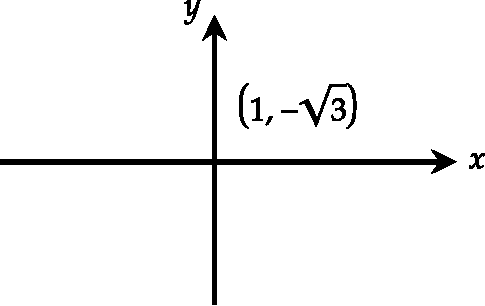
\includegraphics[height=3cm,width=5cm]{CN-Assignment-01}
		\end{figure}
		\begin{align*}
		\text{The magnitude is }|z|&=\sqrt{(1)^{2}+(-\sqrt{3})^{2}}=2\text{ units.}
		\intertext{A complex number in the complex plane is represent by a point.}
		\intertext{The real part is plotted on the $x$-axis and imaginary part on the $y$-axis. hence $z=1-\sqrt{3} i$ can be represented by a point $(1,-\sqrt{3})$ in the complex plane.}
		\end{align*}
		So the correct answers are \textbf{Option (a) and (c)}
	\end{answer}
\item $\left. \right. $		
	\begin{answer}
		\begin{align*}
		z_{1}+z_{2}&=(2+3 i)+(1+2 i)=3+5 i\\
		z_{1}-z_{2}&=(2+3 i)-(1+2 i)=1+i\\
		z_{1} \cdot z_{2}&=(2+3 i) \cdot(1+2 i)=2+4 i+3 i-6 \quad (\text{since} \left.i^{2}=-1\right)\\
		&=-4+7 i\\
		\frac{z_{1}}{z_{2}}&=(2+3 i) \cdot \frac{1}{(1+2 i)}\text{, but} \frac{1}{1+2 i}=\frac{1-2 i}{5}=\frac{1}{5}-\frac{2}{5} i\\
	\text{	hence }\frac{z_{1}}{z_{2}}&=(2+3 i)\left(\frac{1}{5}-\frac{2}{5} i\right)=\left(\frac{2}{5}+\frac{6}{5}\right)+i\left(-\frac{4}{5}+\frac{3}{5}\right)=\frac{8}{5}-\frac{1}{5} i
		\end{align*}
		So the correct answers are \textbf{Option (b), (c) and (d)}
	\end{answer}
\item $\left. \right. $		
	\begin{answer}
 The first three options are true. Option (d) is false as multiplication of two complex number is commutative\\\\
		So the correct answers are \textbf{Option (a), (b) and (c)}
	\end{answer}
\item $\left. \right. $	
	\begin{answer}
		\begin{align*}
		 \text{Let }z&=x+i y,\text{ then }\bar{z}=x-i y\\
		z&=\bar{z} \Rightarrow x+i y=x-i y \Rightarrow 2 i y=0 \text { or } y=0
	\intertext{	Thus $z$ is purely real}
	z+\bar{z}&=0 \Rightarrow x+i y+x-i y=0 \Rightarrow 2 x=0 \Rightarrow x=0
	\intertext{Thus $z$ is purely imaginary}
	\intertext{Any complex number in the complex plane can be written as}
	z&=r(\cos \theta+i \sin \theta)
	\intertext{where $r$ is the modulus of the complex number and $\theta$ is the angle as shown in the figure}
	r&=\sqrt{(1)^{2}+(1)^{2}}=\sqrt{2}\\
	\tan \theta&=\frac{\text { Imaginary part }}{\text { real part }}=\frac{1}{1}=1\\
	\therefore \quad \theta&=\frac{\pi}{4}
	\intertext{Hence the complex number $z=1+i$ can be written as}
	z&=\sqrt{2}\left(\cos \frac{\pi}{4}+i \sin \frac{\pi}{4}\right)
		\end{align*}
	\end{answer}
	
	
	
	
	
	
	
	
	
	
	
	
	
	
	
	
\end{enumerate}